\documentclass[10pt, compress]{beamer}

\usetheme{m}
\usepackage{textcomp}
\usepackage{booktabs}
\usepackage[scale=2]{ccicons}
\usepackage{minted}
\usepackage{smartdiagram}


\usemintedstyle{trac}

\title{Data Management and Introduction to Stata}
\subtitle{}
\date{Thursday 12th April}
\author{David Clark}
\institute{University of Leeds}

\begin{document}

\maketitle

\section{Introductions and Preamble}

\begin{frame}[fragile]
  \frametitle{Introductions}

\textbf{David Clark}
\begin{itemize}
    \item Teaching Fellow in Economics
    
    \item Used Stata for 6(-ish) years ... still learning!
\end{itemize}
    
   \textbf{Kausik Chaudhuri}
\begin{itemize}
    \item  Senior Lecturer in Economics
    
   \item  Used Stata for ..... 
    
\end{itemize}

\end{frame}

\begin{frame}[fragile]
  \frametitle{Who is this course for?}
    Targeted at anyone who has \textbf{no to little} experience using Stata
    
    Primarily for those engaging in \alert{quantitative} research (MRes/PhD)
    
    What to learn to use a statistical package that allows for both use of \textbf{point-and-click GUI} and \textbf{Stata's Markup and Control Language (SMCL)}
      
\end{frame}

\begin{frame}[fragile]
  \frametitle{Who is this course for?}

    For those who want to:
        \begin{itemize}
            \item \textbf{Organise and manage data}
                \begin{itemize}
                    \item Generating, keeping and dropping, reshaping
                \end{itemize}
            \item \textbf{Visualise data}
                \begin{itemize}
                    \item Scatter and line graphs
                    \item Histograms
                \end{itemize}
            \item \textbf{Analyse data}
                \begin{itemize}
                    \item ANOVA
                    \item Regression analysis
                \end{itemize}
            \item \textbf{Automate and reproduce workflow}
                \begin{itemize}
                    \item Log and do-files
                    \item Loops
                \end{itemize}
        \end{itemize}
      
\end{frame}

\section{What is Stata?}

\begin{frame}[fragile]
  \frametitle{What is Stata?}
  Stata is a powerful statistical package with:
  \begin{itemize}

   \item  smart data-management facilities
  
   \item  a wide array of up-to-date statistical techniques
  
   \item  an excellent system for producing publication-quality graphs
    
  \end{itemize}
  
  Available on a variety of operating systems (Windows, Mac OS and Linux distributions)
  
  Also available in different varieties:
  
    \begin{itemize}

   \item  IC (standard)
  
   \item SE (extended)
  
   \item  MP (multiprocessing)
    
  \end{itemize}
  
\end{frame}


\begin{frame}[fragile]
\frametitle{Why not use X?}
There are alternative statistical software packages you can use (to name a few):

\begin{itemize}
    \item R
    \item Matlab
    \item SAS
    \item SPSS
    \item Gauss
    \item Gretl
    \item Eviews
\end{itemize}

\end{frame}

\begin{frame}[fragile]
\frametitle{Crippling Self-Doubt}
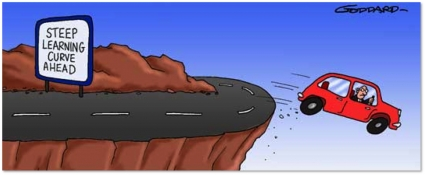
\includegraphics[width=\linewidth,height=\textheight,keepaspectratio]{curve.png}

\end{frame}

\begin{frame}[fragile]
  \frametitle{Stata 14 Front End Graphic User Interface (GUI)}
  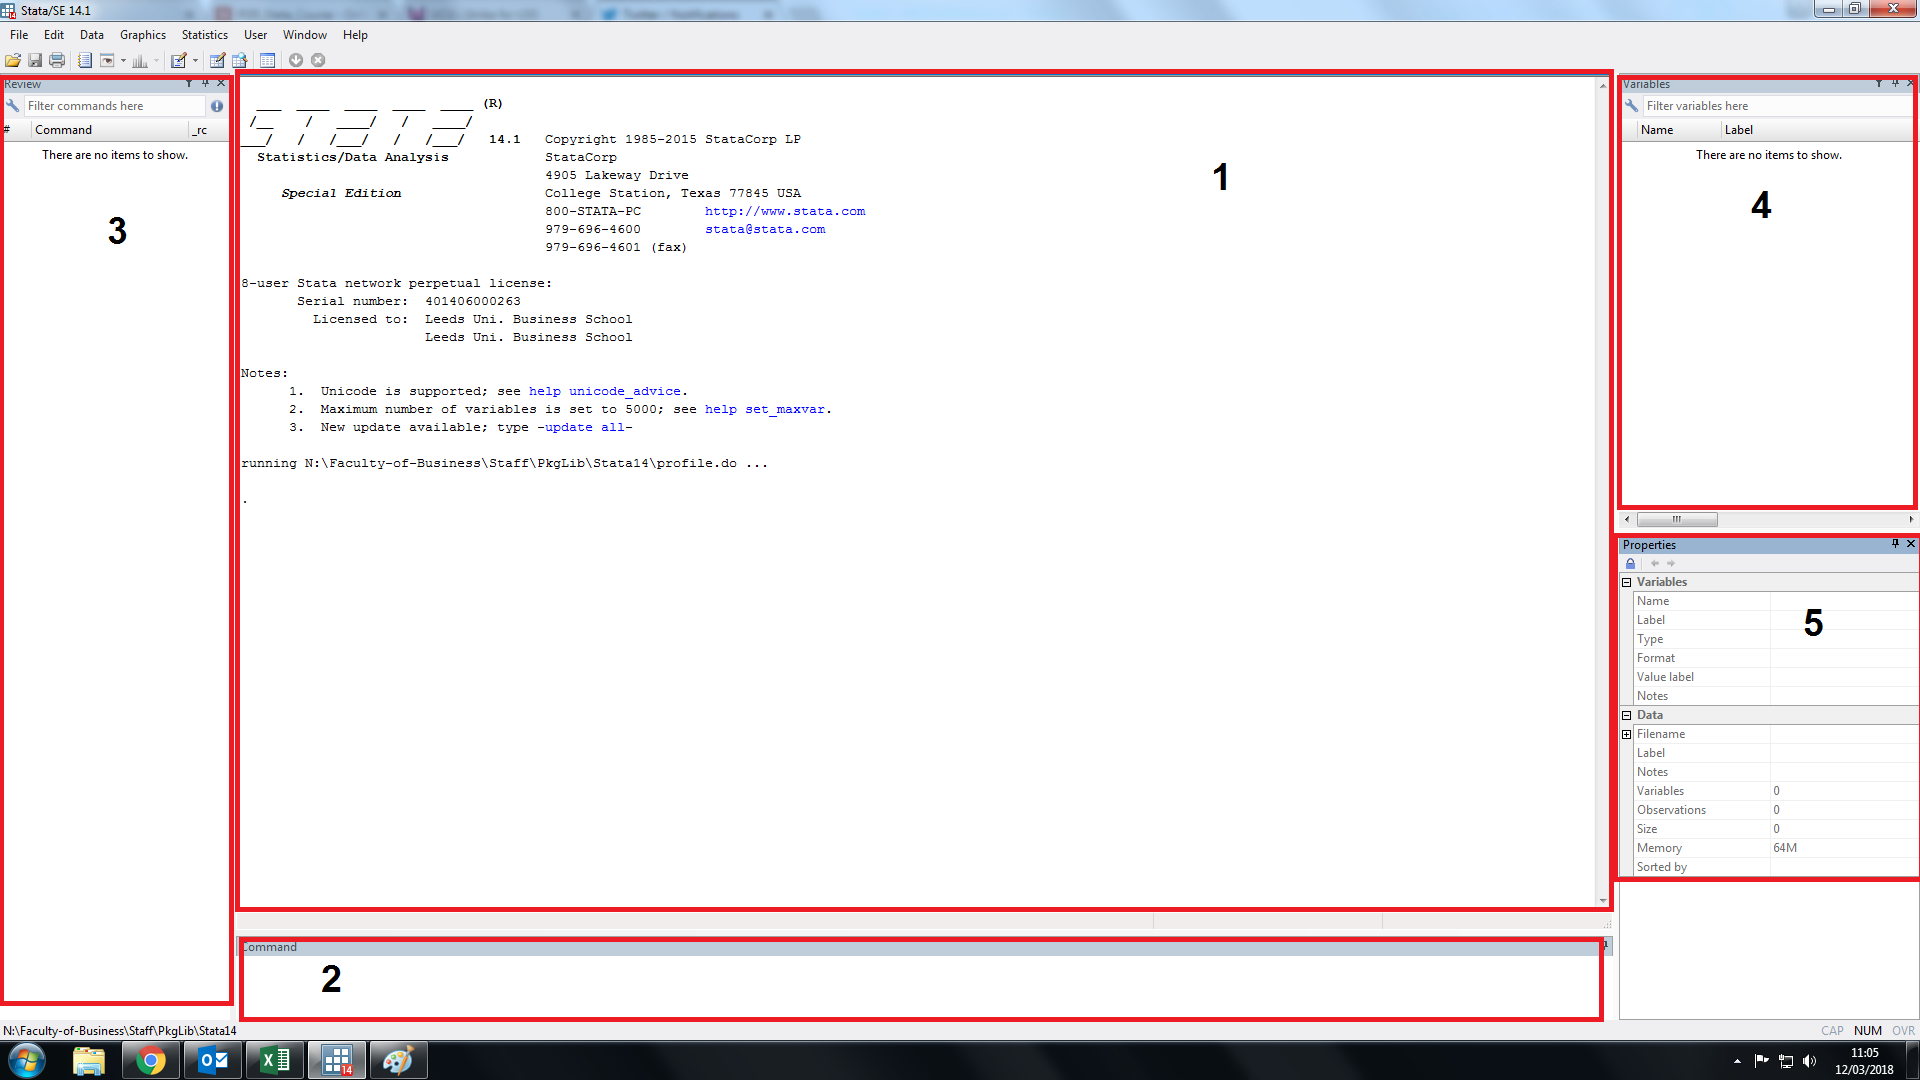
\includegraphics[width=\linewidth,height=\textheight,keepaspectratio]{stata.png}
\end{frame}

\begin{frame}[fragile]
  \frametitle{Stata 14 Front End GUI}
Stata has an menu bar on the top and 5 internal windows.

The \alert{main} window is the one in the middle (1 on the previous slide). It gives
you all the output of your operations in Stata.

The \alert{command window} (2) executes commands. 
\begin{itemize}
    \item You can type commands directly in this window as an alternative to using the menu system.
    \item Stata will show you what the written command is for each action performed using the drop-down menus.
\end{itemize}


\end{frame}

\begin{frame}[fragile]
  \frametitle{Stata 14 Front End GUI}
  
  The \alert{review window} (3), lists all the operations preformed since opening
Stata. If you click on one of your past commands, you will see the command
being displayed in the Command window and you can re-run it by hitting the
enter key.

The \alert{variables window} (4) lists the variables in the current dataset (and their
descriptions). When you double-click on the variable, it appears in the
Command window.

The \alert{properties window} (5) gives information about your dataset and your
variables.

\end{frame}

\section{Stata Workflow}

\begin{frame}[fragile]
\frametitle{Stata Workflow}
\begin{center}
\usetikzlibrary{shapes.geometric} % required in the preamble
\smartdiagramset{module shape=rectangle,
font=\tiny,
module minimum width=2cm,
module minimum height=1cm,
text width=1.7cm,
circular distance=2cm,
circular final arrow disabled=true,
}
\smartdiagram[circular diagram:clockwise]{File management, Data management, Descriptive statistics, Visualisation, Statistical analysis}
\end{center}	
\end{frame}

\newcommand{\insm}{%
\smash{\raisebox{.5\dimexpr3\baselineskip+4\itemsep+2\parskip}{$\left.\rule{0pt}{.5\dimexpr2\baselineskip+2\itemsep+2\parskip}\right\}$\ \parbox{5.5cm}{These two stages will consume the \alert{most time} in any research project}}}
}


\begin{frame}[fragile]
\frametitle{Stata Workflow}
\begin{itemize}
\item \textbf{File management}
\item \textbf{Data management}
\item \textbf{Descriptive statistics} \insm
\item \textbf{Visualisation}
\item \textbf{Statistical analysis}
\end{itemize}
\end{frame}

\section{File Management}

\begin{frame}[fragile]
\frametitle{Stata Workflow: File Management}
\begin{center}
\usetikzlibrary{shapes.geometric} % required in the preamble
\smartdiagramset{module shape=rectangle,
font=\tiny,
module minimum width=2cm,
module minimum height=1cm,
text width=1.7cm,
circular distance=2cm,
circular final arrow disabled=true,
}
\smartdiagram[circular diagram:clockwise]{\textbf{File management}, Data management, Descriptive statistics, Visualisation, Statistical analysis}
\end{center}	
\end{frame}

\begin{frame}[fragile]
\frametitle{File Management}
\begin{itemize}
\item This is often an aspect of using Stata that is \textbf{wrongly} overlooked
\item Usually a facet that people return to after learning the syntax
\item As researchers, \alert{one of our primary objectives}:
\end{itemize}
\begin{center}
	\textbf{Replicability and reliability}
\end{center}
\begin{itemize}
\item If, after testing your research hypothesis, using data, you discover some results of interest, \textbf{what use is this if they cannot be reproduced by others?}
\item Hence, engraining good practices from the beginning, \alert{promotes higher-quality research} in future work
\end{itemize}
\end{frame}

\begin{frame}[fragile]
\frametitle{File Management}
\begin{itemize}
\item What do we mean by \textbf{file management}?
\begin{itemize}
\item Typically, when people (\alert{most}) begin using Stata, they will just open some data and \textbf{do stuff}
\end{itemize}
\item Questions that arise:
\begin{itemize}
\item \textbf{Where is the data stored?}
\item \textbf{Where is the output stored?}
\item \textbf{Where is Stata currently working from?}
\item \textbf{Are we utilising one or many directories?}
\end{itemize}
\item File management is knowing the answer to these questions constantly and having a good justification for their placement
\end{itemize}
\end{frame}

\begin{frame}[fragile]
\frametitle{File Management}
\begin{center}
	\textbf{Where is Stata currently working from?}
\end{center}
\begin{itemize}
\item \alert{Definition}: \textbf{working directory}
\begin{itemize}
\item The (\alert{current}) working directory is the file within the computer's hierarchical file structure that a program is working from
\end{itemize}
\item That is to say, anything you ask Stata to open or to save will be accessed or stored in this working directory
\end{itemize}
\end{frame}

\begin{frame}[fragile]
\frametitle{File Management}
\begin{center}
	\textbf{Where is Stata currently working from?}
\end{center}
\begin{itemize}
\item There are two ways of finding out what the current working directory is in Stata:
\begin{itemize}
\item Look at the bottom-left hand corner of Stata
\end{itemize}
\smallskip
\begin{center}

\includegraphics{pwd1.png}
\end{center}
\begin{itemize}
\item Type the command \textbf{pwd} into the command window in Stata
\end{itemize}
\begin{center}
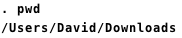
\includegraphics{pwd2.png}
\end{center}
\item Both are telling us that we are working out of the \textbf{Downloads} folder
\end{itemize}
\end{frame}

\begin{frame}[fragile]
\frametitle{File Management}
\begin{itemize}
\item On the University system, this usually is set as a default to the personal drive (M:/)
\item In either case, \textbf{is it a good idea to work out of an indiscriminate folder?}
\begin{itemize}
\item \textbf{Almost always, no!}
\item Why? $\to$ There will be unrelated files that will make it complex to keep track of related files and output
\end{itemize}
So, we have two options what we can proceed with that adhere to \textbf{good practice}:
\begin{itemize}
\item \alert{Change} to a directory that already exists
\item \alert{Create} a directory to work from
\end{itemize}
\end{itemize}
\end{frame}

\begin{frame}[fragile]
\frametitle{File Management: Changing Directory}
\begin{itemize}
\item If the folder that you want to work from \alert{already exists}, we can tell Stata to change the working directory to this folder.
\item For example, imagine I have a folder called \textbf{Thesis$\_$Paper$\_$One} and here is the path (note, this was the file path on my Mac, it will look slightly different on Windows PCs):
\end{itemize}
\begin{center}
\textbf{Users $\to$ David $\to$ Documents $\to$ Projects $\to$ Thesis$\_$Paper$\_$One}
\end{center}
\begin{itemize}
\item This can be done in two ways:
\begin{itemize}
\item Using the drop down menus in the GUI
\item Using the \textbf{cwd} command directly
\end{itemize}
\end{itemize}
\end{frame}

\begin{frame}[fragile]
\frametitle{File Management: Changing Directory}
\textbf{Using the drop down menus in the GUI}
\begin{itemize}
\item If you follow this menu path:
\end{itemize}
\begin{center}
\textbf{File $\to$ Change working directory...}
\end{center}
\begin{itemize}
\item Stata will then open a \alert{file explorer window} where you can navigate to, and choose, the folder you wish to set as the current working directory
\item This is a useful method if \textbf{you do not have the exact file path to hand}
\item Notice, Stata will then print the exact file path in the output window after changing working directory successfully.
\end{itemize}
\end{frame}

\begin{frame}[fragile]
\frametitle{File Management: Changing Directory}
\textbf{Using the drop down menus in the GUI}
\begin{itemize}
\item If you already happen to know the file path to the directory, we can type the change directory command directly into the command prompt:
\end{itemize}
\begin{center}
\mint[fontfamily=tt]{stata}| cd "/Users/David/Documents/Projects/Thesis_Paper_One" |
\end{center}
\textbf{Breakdown}
\begin{itemize}
\item \mint[fontfamily=tt]{stata}|cd| Tells Stata to \textbf{change directory}
\item \mint[fontfamily=tt]{stata}| "/Users/David/Documents/Projects/Thesis_Paper_One" | \textbf{Provides Stata with the file path} to the directory that you will want to change to
\end{itemize}
\end{frame}

\begin{frame}[fragile]
\frametitle{File Management: Creating a Directory}
\begin{itemize}
\item Perhaps you want to create the folder, as part of a new project, which we'll call \textbf{Thesis$\_$Paper$\_$Two}
\item Here, we can only use the command prompt, by typing the following command
\end{itemize}
\begin{center}
\mint[fontfamily=tt, fontsize=\small]{stata}| mkdir "/Users/David/Documents/Projects/Thesis_Paper_Two" |
\end{center}
\textbf{Breakdown}
\begin{itemize}
\item \mint[fontfamily=tt, fontsize=\small]{stata}|mkdir| Tells Stata to \textbf{create a new folder in this directory}
\item \mint[fontfamily=tt, fontsize=\small]{stata}| "/Users/David/Documents/Projects/Thesis_Paper_Two" | \textbf{Provides Stata with the file path} to the directory that you will want to move to (\alert{Projects}) and create a folder in there called \alert{Thesis$\_$Paper$\_$Two}
\end{itemize}
\end{frame}

\section{Demo: Changing and Creating Directories}

\section{Data Management}

\begin{frame}[fragile]
\frametitle{Stata Workflow: Data Management}
\begin{center}
\usetikzlibrary{shapes.geometric} % required in the preamble
\smartdiagramset{module shape=rectangle,
font=\tiny,
module minimum width=2cm,
module minimum height=1cm,
text width=1.7cm,
circular distance=2cm,
circular final arrow disabled=true,
}
\smartdiagram[circular diagram:clockwise]{File management, \textbf{Data management}, Descriptive statistics, Visualisation, Statistical analysis}
\end{center}	
\end{frame}


\begin{frame}[fragile]
\frametitle{Data Management}
\begin{itemize}
\item As stated previously, the data management aspect of the workflow is arguably \textbf{one of the most important (and time-consuming) stages of a research project}
\item \textbf{Why?}
\begin{itemize}
\item Data \alert{might not be native to Stata}, so it must be imported correctly
\item Datasets, particularly survey data, may have some \alert{errors in their reporting and may require our attention}
\item You may want to gather data from different datasets and \alert{consolidate them into one master dataset}
\item Perhaps you want to \alert{create new variables} based on the original data
\end{itemize}
\item Taking the time to carry out this stage properly will \textbf{save you time in the long run}
\end{itemize}
\end{frame}

\begin{frame}[fragile]
\frametitle{Data Management: Importing Data}
We can characterise datasets into two broad sets:
\begin{itemize}
\item \textbf{Stata datafiles} (.dta files)
\begin{itemize}
\item This is the file type that Stata can read and work with \alert{natively}; as such it requires little work to open
\end{itemize}
\item \textbf{All other types of datafile}
\begin{itemize}
\item This is a huge set but these have to imported as a \alert{foreign} datafile
\item While the list is endless, we will focus only on:
\begin{itemize}
\item CSV
\item XLS
\item XLSX
\end{itemize}
\end{itemize}
\item If there are other datasets from particular programs you'd like to import, consider the program \textbf{StatTransfer - \alert{not free}}
\end{itemize}
\end{frame}

\begin{frame}[fragile]
\frametitle{Data Management: A Quick Aside}
Before we go ahead and learn to import and open different datafile types into Stata, \textbf{we need to make sure we're working on a blank canvas}, so to speak
If we don't do this beforehand:
\begin{enumerate}
\item Stata will \textbf{refuse} to open other data as it will risk losing data that is already in memory
\item It may, in theory, \textbf{corrupt} the imported data and/or the data in current memory
\end{enumerate}
So to avoid the risk of either of the two above outcomes, \textbf{we type in the following command into Stata before importing anything}:
\begin{center}
\mint[fontfamily=tt]{stata}|clear all|
\end{center}
This will \alert{clear literally everything from Stata's working memory}, including, most importantly, any open datafiles
\end{frame}

\begin{frame}[fragile]
\frametitle{Data Management: Importing Stata Datafiles}
\textbf{Stata datafiles} (.dta files)
\begin{itemize}
	\item As previously stated, these are native to Stata and so are very easily open and read by Stata
	\item \textbf{Assuming that the datafile is stored in the current working directory}, use the following drop down menu path:
\end{itemize}
\begin{center}
\textbf{File $\to$ Open}
\end{center}
\begin{itemize}
	\item Once you've done this, you can navigate to the datafile and then double-click to open
	\item An easy way to verify the data is now loaded into to Stata is to check the \alert{variables window}
	\item If you see variables names in there, \alert{you've successfully opened your Stata datafile}
\end{itemize}
\end{frame}

\begin{frame}[fragile]
\frametitle{Data Management: Importing XLS/X Datafiles}
\textbf{Excel datafiles} (.xls/x files)
\begin{itemize}
	\item Despite secondary data being provided in a .dta format more frequently - \textbf{it is more common for the data to be provided as an Excel file} (either .xls or .xlsx file types)
	\item This is not quite as strightforward as opening a .dta file but it is luckily not too complex an operation
	\item \textbf{Assuming that the datafile is stored in the current working directory}, use the following drop down menu path:
\end{itemize}
\begin{center}
\textbf{File $\to$ Import $\to$ Excel Spreadsheet (*.xls;*.xlsx)}
\end{center}
\end{frame}

\begin{frame}[fragile]
\frametitle{Data Management: Importing XLS/X Datafiles}
 After following the drop-down path, you'll be presented with the following window:
\begin{center}
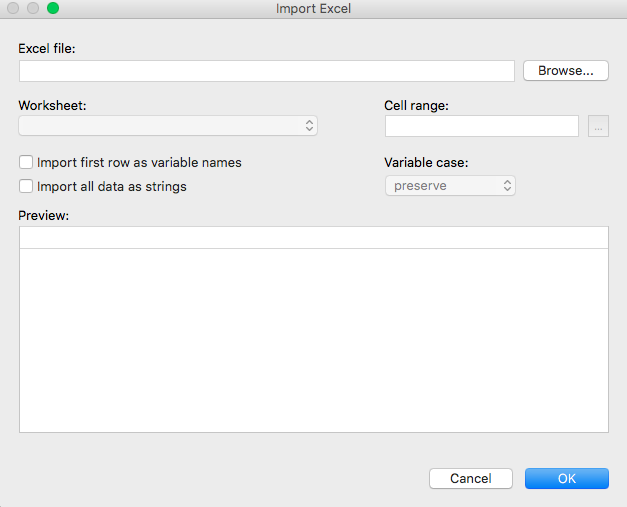
\includegraphics[width=7cm,height=6cm,keepaspectratio]{xls.png}
\end{center}
\end{frame}

\begin{frame}[fragile]
\frametitle{Data Management: Importing XLS/X Datafiles}
Complete the following steps to import the datafile:
\begin{enumerate}
	\item Direct Stata to the datafile by selecting \textbf{Browse..}
	\item Choose the worksheet that your data is in within the workbook
	\item Typically, the heading of each column of the spreadsheet will contain the variable name. Select the option, \textbf{Import first row as variable names}
	\item In the preview pane at the bottom of the window, you can confirm here that the data is being imported correctly
	\item Finally, press OK and Stata should have then successfully imported the Excel datafile
\end{enumerate}
\end{frame}

\begin{frame}[fragile]
\frametitle{Data Management: Importing CSV Datafiles}
\textbf{Comma-Seperate Values datafiles} (.csv files)
\begin{itemize}
	\item Other than Excel datafile types, another popular datafile format is the comma-seperate values (CSV) datafiles
	\item They're popular as they \alert{do not require proprietary software to open or edit}
	\item \textbf{Assuming that the datafile is stored in the current working directory}, use the following drop down menu path:
\end{itemize}
\begin{center}
\textbf{File $\to$ Import $\to$ Text data (delimited;*.csv)}
\end{center}
\end{frame}

\begin{frame}[fragile]
\frametitle{Data Management: Importing CSV Datafiles}
 After following the drop-down path, you'll be presented with the following window:
\begin{center}
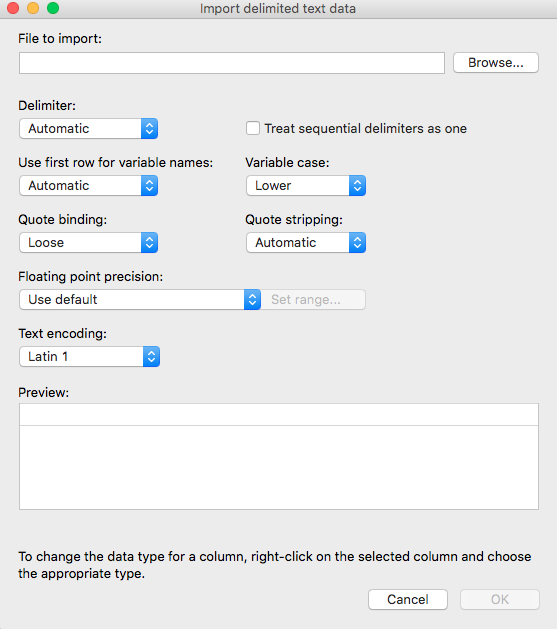
\includegraphics[width=6cm,height=8cm,keepaspectratio]{csv.png}
\end{center}
\end{frame}

\begin{frame}[fragile]
\frametitle{Data Management: Importing CSV Datafiles}
Complete the following steps to import the datafile:
\begin{enumerate}
	\item Direct Stata to the datafile by selecting \textbf{Browse..}
	\item Choose the delimiter (the symbol that Stata recognises as separating individual data observations) - automatic is usually best
	\item Just in the case with XLS/X files, if the first row represents the variable names, choose always under the appropriate option
	\item Observe the preview and if everything looks in its proper format, press OK 
\end{enumerate}
\end{frame}

\section{Demo: Importing Datafiles}

\section{Browsing and Manipulating Data}

\begin{frame}[fragile]
\frametitle{Browsing and Manipulating Data}
So, regardless of how your data had been stored originally, \textbf{you should be aware} of how to import the datafile into Stata

\begin{center}
\alert{Now what?}	
\end{center}

\begin{center}
\textbf{This is where we get started with Stata!}	
\end{center}

What might you want to do immediately after importing data?
\begin{enumerate}
	\item Browse the data
	\item Edit the data
	\item Generate new variables  
\end{enumerate}
Keep in mind, before we've imported and formatted the data correctly, \textbf{we should not be embarking on any type of statistical analysis}
\end{frame}

\begin{frame}[fragile]
\frametitle{Browsing Data}
Despite the fact we saw a preview of the data when importing CSV/XLS datafiles, we don't really know how the data looks\\

Something we can do is \alert{browse} the dataset by simply typing:

\begin{center}
\mint[fontfamily=tt]{stata}|browse|
\end{center}

When you do so, you should see the following window open on your screen...

\end{frame}

\begin{frame}[fragile]
\frametitle{Browsing Data}
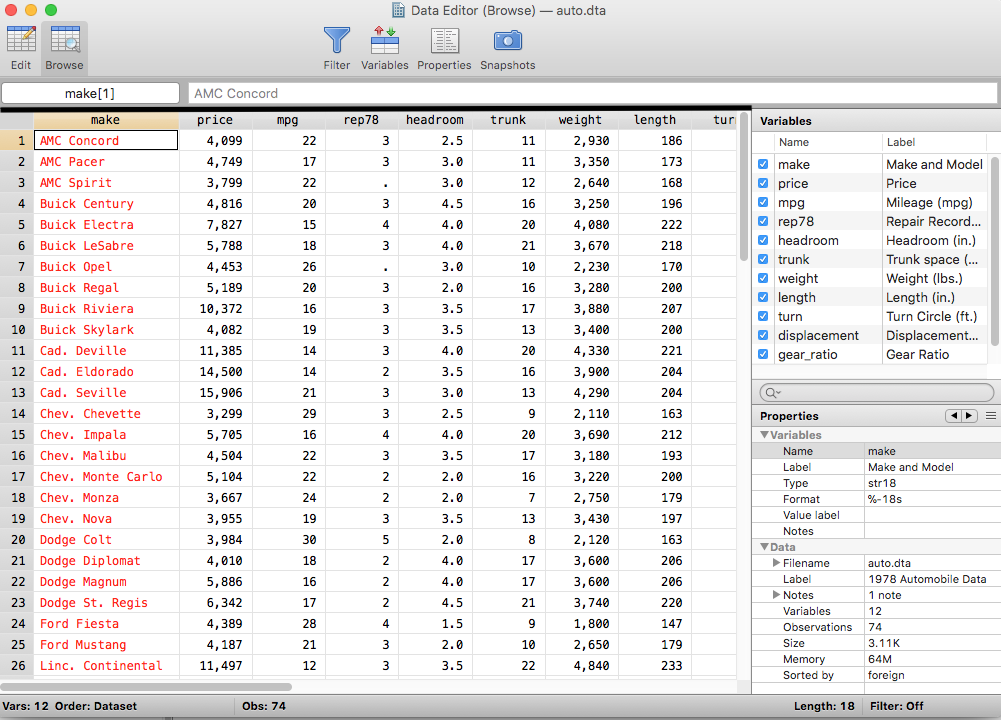
\includegraphics[width=\linewidth,height=\textheight,keepaspectratio]{browse.png}
\end{frame}

\begin{frame}[fragile]
\frametitle{Browsing Data}
That's great but \textbf{what's going on in this huge window?}
\begin{enumerate}
\item \textbf{Main window}
\begin{itemize}
	\item This is main data browser pane within the browse window
	\item Here, we can see all our \textbf{variables and the observations for each individual unit in the dataset} (\alert{notice some are in red? We'll come back to this})
\end{itemize}
\item \textbf{Top-right corner}
\begin{itemize}
	\item This is the \textbf{variables pane}
	\item Here you can see each of the variables within the dataset as well as their label
	\item You can (un)tick them to filter the data in the browser pane
\end{itemize}
\item \textbf{Bottom-right corner}
\begin{itemize}
	\item This is the \textbf{properties} pane
	\item It displays information about the selected variable - notably the \textbf{variable type}
\end{itemize}	
\end{enumerate}

\end{frame}

\begin{frame}[fragile]
\frametitle{A Quick Aside - Variable Types}
In the last window, you've probably noticed that the observations for the variable \alert{make} were all in \textbf{red}, whilst the others were just in \textbf{black} text

\begin{center}
\alert{Any ideas why?}	
\end{center}

We could go into \textbf{a lot} of detail about this but simply put:
\begin{itemize}
	\item When you see the observations of a variable in \textbf{red}, this signifies that the variable is of type \textbf{string} - that's to say the data is a word or contains text
	\item Otherwise, when the data is in black, this usually signifies that data is stored as a \textbf{numeric type} (e.g. \alert{float, integer, double})
\end{itemize}

\end{frame}

\begin{frame}[fragile]
\frametitle{Manipulating Data: Editing}
When it comes to \textbf{manipulating/changing the data}, for whatever reason, there are a few ways of doing this:

\begin{enumerate}
\item Editing the data within the browser directly (\textbf{not recommended})
\begin{itemize}
\item \alert{Why?} $ \to\ $ piecemeal changes of the data doesn't speak to \textbf{replicability and reliability}
\end{itemize}
\item Using a suite of commands that allow you to change aspects of a variable (\textbf{recommended}) - these include: 
\begin{itemize}
\item \mint[fontfamily=tt]{stata}|rename| - renaming variables
\item \mint[fontfamily=tt]{stata}|keep| - keep a variable or observations in a range
\item \mint[fontfamily=tt]{stata}|drop| - drop a variable or observations in a range
\item \mint[fontfamily=tt]{stata}|generate| - create a new variable
\end{itemize}
\end{enumerate}

\end{frame}

\begin{frame}[fragile]
\frametitle{Manipulating Data: Renaming and Labelling Variables}
\underline{\textbf{Renaming variables:}}\\
\alert{Syntax}
\begin{center}
\mint[fontfamily=tt]{stata}|rename [oldname] [newname]|
\end{center}
\alert{Example}
\begin{center}
\mint[fontfamily=tt]{stata}|rename year Year|
\end{center}
\underline{\textbf{Labelling variables:}}\\
\alert{Syntax}
\begin{center}
\mint[fontfamily=tt]{stata}|label variable [varname] "[label]"|
\end{center}
\alert{Example}
\begin{center}
\mint[fontfamily=tt]{stata}|label variable Year "Year survey took place"|
\end{center}
\end{frame}

\begin{frame}[fragile]
\frametitle{Manipulating Data: Keeping and Dropping Variables}
\begin{itemize}
\item The original dataset may contain variables you are \textbf{not interested in} or \textbf{observations you don't want to analyse} 
\item It's a good idea to get rid of these first - that way, they won't use up valuable memory and these data will not inadvertently be included into your statistical analysis
\item This can be done using either:
\begin{itemize}
\item \mint[fontfamily=tt]{stata}|keep|
\item \mint[fontfamily=tt]{stata}|drop|
\end{itemize}
\end{itemize}
\alert{Syntax (applies to drop also)}
\begin{center}
\mint[fontfamily=tt]{stata}|keep [varlist] |
\end{center}
\alert{Example}
\begin{center}
\mint[fontfamily=tt]{stata}|keep id age year health|
\end{center}
\end{frame}

\begin{frame}[fragile]
\frametitle{Manipulating Data: Keeping and Dropping Variables}
\begin{itemize}
\item The previous slide shows the most straightforward implementation of the \alert{keep and drop} commands, however we can make these commands more complex by using what are called \textbf{relational} and \textbf{logical operators}
\item This is a better alternative to piecemeal edits to the data, as \textbf{you can set particular conditions to which data is kept or dropped} given your own research ideals
\item While you may not use all of them, the next slide lists all the available operators that \textbf{you can use with commands in Stata that have the option of setting a conditional}
\end{itemize}
\end{frame}

\begin{frame}[fragile]
\frametitle{Relational and Logical Operators}
  \begin{columns}[onlytextwidth]
    \column{0.5\textwidth}
      \textbf{Relational}
      \begin{itemize}
\item \mint[fontfamily=tt]{stata}|==| equal to
\item \mint[fontfamily=tt]{stata}|!=| not equal to
\item \mint[fontfamily=tt]{stata}|>| greater than
\item \mint[fontfamily=tt]{stata}|>=| greater than or equal to
\item \mint[fontfamily=tt]{stata}|<| less than
\item \mint[fontfamily=tt]{stata}|<=| less than or equal to
      \end{itemize}

    \column{0.5\textwidth}
     \textbf{Logical}
      \begin{itemize}
     \item  \mint[fontfamily=tt]{stata}|&| and
	\item \mint[fontfamily=tt]{stata}||| or
	\item \mint[fontfamily=tt]{stata}|~| not
	\item \mint[fontfamily=tt]{stata}|!| not
      \end{itemize}
  \end{columns}
\end{frame}

\begin{frame}[fragile]
\frametitle{Manipulating Data: Using Conditionals}
It may seem like it's starting to get complicated now but this is a really small addition

For example, the \alert{general syntax} for \alert{keep} is as follows:

\begin{center}
\mint[fontfamily=tt]{stata}|keep [varlist] if [condition] |
\end{center}

This addition at the end of the \alert{required} syntax is applicable to \textbf{most} Stata commands

A good way to check is to type \mint[fontfamily=tt]{stata}|help [command]|

This will bring up a help file for a given command (\alert{and is very useful!})

\end{frame}

\section{Demo: Using Conditionals}

\section{Descriptive Statistics}

\begin{frame}[fragile]
\frametitle{Stata Workflow: Descriptive Statistics}
\begin{center}
\usetikzlibrary{shapes.geometric} % required in the preamble
\smartdiagramset{module shape=rectangle,
font=\tiny,
module minimum width=2cm,
module minimum height=1cm,
text width=1.7cm,
circular distance=2cm,
circular final arrow disabled=true,
}
\smartdiagram[circular diagram:clockwise]{File management, Data management, \textbf{Descriptive statistics}, Visualisation, Statistical analysis}
\end{center}	
\end{frame}

\begin{frame}[fragile]
\frametitle{Descriptive Statistics}
	It may seem like we've go though a lot to get to this point but again, 
	\alert{thorough procedure pays off}
	
	Up to this point, we should be able to:
	
	\begin{itemize}
		\item Set working directories for new projects
		\item Import various datafiles
		\item Manipulate data and generate new variables
	\end{itemize}
	
	\textbf{Only now} should we proceed with looking at and analysing the data, \textbf{not before!}
\end{frame}

\begin{frame}[fragile]
\frametitle{Descriptive Statistics}
So, what do we mean by \textbf{descriptive statistics}? 

These include but \alert{are not limited to}:

\begin{itemize}
\item Sample size
	\begin{itemize}
		\item Overall
		\item Sub-group
	\end{itemize}
\item Outcome frequencies
\item Measures of central tendency
	 \begin{itemize}
		\item Mean
		\item Median
		\item Mode
	\end{itemize}
\item Measures of variability
	 \begin{itemize}
		\item Standard deviation
		\item Variance
	\end{itemize}
\item Variable relation
	 \begin{itemize}
		\item Correlation
	\end{itemize}
\end{itemize}

\end{frame}

\begin{frame}[fragile]
\frametitle{Descriptive Statistics}
Some of you (hypothetically) may ask, \alert{"What's the point in these descriptive statistics?"}

Short answer: \textbf{A LOT!}

It can tell us:

\begin{itemize}
\item The dimensions of the dataset
\item What the distribution is of each variable
\item How variables are related with one another and to what degree
\end{itemize}

The reason that these are important before modelling is because a lot about what we want to know about the data between groups or within groups are expressed here!

\end{frame}

\begin{frame}[fragile]
\frametitle{Descriptive Statistics}

These properties of the data are attained using a few key commands in Stata:

\begin{itemize}
 \item \mint[fontfamily=tt]{stata}|describe|  \alert{"describes" the data}
 \item 	\mint[fontfamily=tt]{stata}|summarize|  \alert{summarises the data}
 \item  \mint[fontfamily=tt]{stata}|tabulate|  \alert{tabulates a/the variable(s)}
 \item \mint[fontfamily=tt]{stata}|correlate| \alert{creates a correlation matrix of specified variables}  
\end{itemize}

\end{frame}

\begin{frame}[fragile]
\frametitle{Descriptive Statistics: Describe}

\begin{center}
\mint[fontfamily=tt]{stata}|describe [varlist], [options] |
\end{center}

This reports some basic information about the dataset and its variables (size, number of variables and observations, storage types of variables etc.

Notice, there is the ability to add an option to the end of the command - \alert{These are option but may be useful}
\begin{itemize}
\item \mint[fontfamily=tt]{stata}|simple| display only variable names
\item \mint[fontfamily=tt]{stata}|short| display only general information
\item \mint[fontfamily=tt]{stata}|fullnames| do not abbreviate variable names
\item \mint[fontfamily=tt]{stata}|numbers| display variable number along with name
\end{itemize}
\end{frame}

\begin{frame}[fragile]
\frametitle{Descriptive Statistics: Summarize}

\begin{center}
\mint[fontfamily=tt]{stata}|summarize [varlist] if [condition], [options] |
\end{center}

\alert{summarize} calculates and displays a variety of univariate summary statistics. If no \alert{varlist} is specified, summary statistics are calculated for all the variables in the dataset

The main option that can be used here is \alert{detail}, which will produce additional summary statistics, such as \alert{third and fourth-order moments - skewness and kurtosis} 

Notice, the \textbf{conditional option} is available here, which \textbf{allows for summary statistics for a sub-sample of the data}

\end{frame}

\begin{frame}[fragile]
\frametitle{Descriptive Statistics: Tabulate}

The \alert{general syntax} for \alert{tabulate} is as follows:

\begin{center}
\mint[fontfamily=tt]{stata}|tabulate [varlist] if [condition], [options] |
\end{center}

\alert{tabulate} produces a one(two)-way table of frequency counts

Again, there is the option to \textbf{tabulate the data on a condition} that you specify about the data

There are options here but they are \alert{used infrequently}, so the standard syntax is \alert{usually} enough
\end{frame}

\begin{frame}[fragile]
\frametitle{Descriptive Statistics: Correlate}

\begin{center}
\mint[fontfamily=tt]{stata}|correlate [varlist] if [condition], [options] |
\end{center}

The \alert{correlate} command displays the correlation matrix or covariance matrix for a group of
variables. If \alert{varlist is not specified}, the matrix is displayed for \alert{all variables} in the dataset.

Again, there is the option to \textbf{look at correlations between variables on a condition} that you specify about the data

Moreover, like tabulate, there are options here but they are \alert{used infrequently}, so the standard syntax is \alert{usually} enough

\end{frame}

\section{Demo: Descriptive Statistics} 

\plain{}{Questions?}

\end{document}
